\documentclass[a4paper,11pt]{article}
\input{/home/tof/Documents/Cozy/latex-include/preambule_lua.tex}
\newcommand{\showprof}{show them}  % comment this line if you don't want to see todo environment
\fancyhead[L]{TP Dessiner avec Turtle}
\newdate{madate}{10}{09}{2020}
\fancyhead[R]{Première - NSI} %\today
\fancyfoot[L]{~\\Christophe Viroulaud}
\fancyfoot[C]{\textbf{Page \thepage}}
\fancyfoot[R]{\includegraphics[width=2cm,align=t]{/home/tof/Documents/Cozy/latex-include/cc.png}}

\begin{document}
\begin{Form}
\section{Les bibliothèques}
\subsection{Présentation}
Pour faciliter le travail des codeurs, il existe des outils spécialisés dans diverses tâches. On les appelle \emph{bibliothèques}, \emph{modules} ou encore \emph{librairies}. Comme son nom l'indique la bibliothèque \emph{math} offre des fonctionnalités permettant d'effectuer des calculs mathématiques.
\subsection{Documentation}
Il n'est pas nécessaire de connaître par cœur toutes les possibilités de chaque librairie. Il est par contre indispensable de savoir utiliser la documentation en ligne de Python.
\begin{activite}
\begin{enumerate}
\item Se rendre sur la page \url{https://docs.python.org/3/}
\item Sélectionner la langue et la version de Python correspondante à l'EDI utilisé.
\item Dans la barre de recherche, taper \emph{math} et ouvrir le premier lien.
\item Chercher la fonction permettant de calculer la racine carrée d'un nombre.
\end{enumerate}
\end{activite}
\subsection{Utilisation}
Pour utiliser les fonctionnalités proposées par une bibliothèque, il faut d'abord l'importer dans le programme. Plusieurs possibilités d'import existent:
\begin{lstlisting}
# importe toute la bibliothèque
import math
# calcule le cosinus de l'angle (en radians)
c = math.cos(0.5)
\end{lstlisting}
\begin{lstlisting}
# importe toute la bibliothèque et lui donne un alias
import math as m
c = m.cos(0.5)
\end{lstlisting}
\begin{lstlisting}
# importe toutes les fonctions de la bibliothèque
from math import *
# Il ne faut plus faire référence au nom de la bibliothèque
c = cos(0.5)
\end{lstlisting}
\begin{lstlisting}
# n'importe que les fonctions nécessaires dans le programme
from math import cos
# Il ne faut plus faire référence au nom de la bibliothèque
c = cos(0.5)
\end{lstlisting}
\section{Une bibliothèque graphique}
\subsection{Découverte}
La bibliothèque \emph{turtle} est un module simple pour réaliser des figures géométriques. La \emph{tortue} avance, tourne sur l'écran et trace les traits demandés par l'utilisateur.
\subsection{Premiers déplacements}
Les possibilités sont nombreuses. Il faut d'abord découvrir quelques déplacements.
\begin{activite}
\begin{enumerate}
\item Dans la documentation, chercher le rôle des fonctions:
\begin{itemize}
\item forward(), backward()
\item left(), right()
\item up(), down()
\end{itemize}
\item Tracer un carré de 100 de côté.
\end{enumerate}
\end{activite}
\subsection{Des figures plus complexes}
\begin{activite}
\begin{enumerate}
\item Réaliser la figure \ref{carres}.
\item Remplir chaque carré avec une couleur, de la manière suivante:
\begin{itemize}
\item rouge si le numéro du carré tracé est impair,
\item vert s'il est pair.
\end{itemize}
\end{enumerate}
\end{activite}
\begin{figure}[!h]
\centering
\includegraphics[width=8cm]{ressources/carres.png}
\captionof{figure}{Des carrés et des rotations}
\label{carres}
\end{figure}


\end{Form}
\end{document}